\documentclass{aamas2014}
\usepackage{graphicx}

\title{Stereotypes in Coordination Domains}
\author{Carrie Rebhuhn \\
Oregon State University \\
rebhuhnc@onid.orst.edu
 \and Kagan Tumer \\
 Oregon State University \\ 
 kagan.tumer@oregonstate.edu
 }
\begin{document}
\maketitle

\begin{abstract}
In coordination tasks with heterogeneous agents it can be critical to have a representation of another agent's abilities. However in large systems it is impossible to keep a complete model of other agents. We show that in coordination tasks, using a generalized agent model, or \emph{stereotype}, can increase the performance of an agent. We demonstrate this in an n-agent pursuit domain as well as a rover POI surveillance domain.

\vspace{1in}

\end{abstract}

\section{Introduction}

%TODO: this is a harsh intro?
Many multiagent problems treat other agents as background noise, insensitive to the differences between them. In some cases this approach makes sense, as the actions of agents are decoupled enough that they do not need to consider the action of its collaborators. In domains with higher coupling and coordination requirements, knowledge of an agent's action preferences or capability differences should influence other agents' decision-making process.


Agent modeling techniques accommodate these differences. Early work focused on modeling the actions of other agents in order to predict and exploit their next move. However this approach comes at a considerable cost when encountering more than one other agent. If a multiagent system is large, it can become costly for each agent to create a separate model of another agent. Modeling each agent individually can also hinder performance if an agent has brief interactions with another agent in the system, and cannot take advantage of the model.

An approach which has had more success on larger systems is the approach of \emph{generalized} agent modeling \cite{GOM}. This approach dictates a fundamental set of agent models, and each agent in the system is fitted to one of these model. This becomes much more scalable because the number of models in the system does not grow with the number of agents. This also allows model information to be used on any agent, whether encountered previously or not, with a given confidence about an agent's type identification. However this approach requires prior knowledge about the structure of models existing in the system. This can lead to issues in identifying coordinating actions if there are unmodeled behaviors, and leaves no room to accommodate adaptation within the agent type.

We demonstrate learning gains using an abstract type identification. Instead of incorporating an explicit model defined by a type of agent and then reasoning about each agents in the environment, we simply identify each agent with a capability type, and then incorporate this information into the state space of the agent. We demonstrate the efficacy of this approach in two domains; a pursuit domain and a rover domain. This demonstrates the efficacy of using high-level type information while being able to scale to much larger systems.

Our approach has the advantages of:
\begin{itemize}
\item \textbf{Simplicity}: We show that by including even an abstract identification of type in the state space, we can leverage information about agents. This allows the use of any classifier. We demonstrate that classification techniques can be leveraged in simple learning without concept reasoning about the state representation.

\item \textbf{Scalability}: Unlike traditional game theoretic representations, the optimal joint action does not need to be calculated. Our approach uses a very abstract identification of types (which is represented by the ratio of types in the different quadrants). This input is able to scale with the number of agents without increasing the complexity of the state space.

\item \textbf{Graceful Degradation}: In many approaches using agent modeling, if an agent misidentifies a type it may reason incorrectly about its most desirable coordination action and may make a severe mistake. Because our approach uses an adaptive model (a neural network) the potential for incorrectly identifying is implicitly considered, therefore minimizing the cumulative effect of mistaken identifications.

\end{itemize}

Because of these contributions we can extend the use of agent modeling in large domains where it has previously been computationally intractable.

The paper is structured as follows: Section \ref{sec:relatedwork} outlines related work on agent modeling and coordination domains. Section \ref{sec:experimental} describes the method we use for our experiments. Section \ref{sec:results} discusses the findings of our experiments, and Section \ref{sec:discussion} discusses the implications of our results and directions for future work.


\section{Related Work}
\label{sec:relatedwork}

Stereotyping has varying definitions. We define it as grouping several agents under a single model definition. By identifying another agent's policy, an agent can make a more informed decision. The  origins of stereotyping lie in agent modeling, which we overview in Section \ref{sec:agentmodeling}. We then discuss stereotypes in Section \ref{sec:stereotyping}. We give background on neural evolution and the pursuit domain in Section \ref{sec:neuroevo}. We also give a brief background on the rover domain in Section \ref{sec:rover}.

\subsection{Agent Modeling}
\label{sec:agentmodeling}

It is intuitive that knowing information about your opponent could give some advantage against them, but the real question is how to compactly represent this with enough detail to gain maximum advantage. Early work in poker produced two algorithms using agent modeling with his \emph{Loki} poker-playing program, Generic Opponent Modeling (GOM) and Specific Opponent Modeling (SOM) which keep track of probabilities that each player will play a hand and continuously update these. GOM did not differentiate between the poker players, while SOM created a model for each player. GOM and SOM proved able to outperform algorithms without modeling \cite{Loki}.

Chakraborty et al. models memory-bounded agents using high-level features derived from a fixed number of past actions called Targeted Opponent Modeling for MEmory-Bounded Agents (TOMMBA) \cite{TOMMBA}. Ponsen et al. propose a Bayes-relational opponent model that starts with a set of priors also, but then use this to learn a relational regression tree to adapt these to specific opponents \cite{Ponsen}. Williams et al. determine when to make concessions by using a Gaussian process to estimate the future play of an opponent \cite{Williams}. Early work by Carmel et al. develops an extension to $L^*$ by approaching modeling agents as a dimensional reduction of a deterministic finite automaton (DFA), and then uses this model to predict and exploit its next action \cite{Carmel}.

Training examples are used from previous plays to train the classifier. The classifier then takes state information as a feature vector and returns the predicted output action. Ekmekci and Sirin use three different machine learning techniques; neural networks, support vector machines, and K nearest neighbors, in order to classify opponent moves in poker \cite{Ekmekci}. Laviers et al. used an SVM classifier to classify plays in Rush Football based on a set of starting configurations and offensive and defensive plays \cite{Laviers}. They construct the Rush Football into a supervised learning problem and trained the classifier to learn an opponent's defensive plays from a set of spatiotemporal features.

Statistical and classification approaches are useful in the fact that they do not require extensive reasoning about another agent's actions. Statistical methods also adapt quickly to changes in the agent's strategy, and classifiers are often able to model underlying complex functions in an agent's behavior. However, these approaches also have drawbacks. Classifiers typically require a large dataset for training. Also, predictive models do not always generalize well to previously unseen opponents \cite{predictivemodels}. Additionally, a player's recent history may not always be a good predictor of playing style \cite{playingstyle}.

Uncertainty is also a large factor in playing poker. Southey et al. use a Bayesian probabilistic model to separate the uncertainty in game dynamics from the uncertainty in opponent type identification. Bard and Bowling mitigate the game uncertainty by using a Rao-Blackwellized particle filter in poker to identify the opponent's state as well as a model of its playing dynamics \cite{Southey,Bard}.


\subsection{Stereotyping}
\label{sec:stereotyping}

These are all ways of learning an opponent's strategy, but few scale well to a large number of agents. If the agent types are known, however, it is possible to fit them to a specific type. Teofilo et al. show that a Q-learning agent whose state incorporated predefined player types, which were calculated based on the frequency of past plays, outperformed basic/intermediate playing strategies. Felix and Reis automatically classify opponents based on tehir VP\$IP (voluntary money in pot) and their AF (aggression factor) into four distinct categories: loose passive, loose aggressive, tight passive, and tight aggressive \cite{Teofilo}.

Lockett identifies several `cardinal opponents', which are pre-defined models that describe all dimensions of a player's actions. They then use NEAT to evolve a `Mixture Identifier', which classifies agents in terms of these cardinal opponents \cite{Lockett}. Particle filters have been also used in Fictitious Play to track switching between a fixed number of strategies represented as Hidden Markov Models.

These techniques focus on either building a model of each of your opponents, or relying on a set of predefined models. Modeling each of your opponents does not scale well when you have many opponents that need separate models for each. Relying on a set of predefined models gets around this problem, but wholly rejects the potential for adaptation of agents. We take a step away from these approaches, and instead use a simple identification of abilities rather than to predict actions. This allows the adaptation to be handled by the evolutionary framework rather than by adjusting models.

There are several current approaches to the implementation of the stereotyping concept. Stereotyping has been combined with the concept of `trust' using a tree model to represent a stereotype, and these stereotypes are shared and updated by the agent community \cite{burnett2010bootstrapping}. This is further developed by the concept of \emph{stereotypical reputation}, which gives a mechanism by which agents that have no set opinion can use the opinions developed by others in the system through \emph{stereotypes} \cite{burnett2013stereotypical}. Denzinger and Hamdan use stereotypes with a periodic reevaluation of the chosen stereotype, and may switch between different stereotypes \cite{denzinger2004improving}. Bard and Bowling present a method of learning robust responses to several player types learned offline, which provides implicit modeling rather than relying on an explicit model of an agent's actions \shortcite{DBLP:conf/aaai/BardB07}.


\subsection{NeuroEvolution}
\label{sec:neuroevo}

Neuroevolution is a guided search technique that applies evolutionary principles to neural networks in order to adapt them to a problem. Neural networks are used as function approximators where the scaled values of the state elements are given as inputs, and the outputs correspond to action elements. The general algorithm used in neuroevolution is given as:

\begin{enumerate}
\item Generate $k$ new population members through mutation operations.
\item Obtain fitness values for each population member by simulation.
\item Keep the $k$ population members with the highest fitness.
\end{enumerate}

This is the neuroevolution algorithm that we use in this work.

Neuroevolution has been used often in the pursuit domain, particularly using coevolution \cite{panait,otherpursuitpaper}. The pursuit game traditionally consists of four predators and one prey on a gridworld.

\section{Experimental Setup}
\label{sec:experimental}

Our experiments are performed on the n-agent pursuit game. This game is focused pursuers pursuing a prey agent. Traditionally the game is played with four agents pursuing one prey. However, because we wanted to test the scalability of our algorithm we extended the traditional approach in \ref{predprey} to accommodate any number of agents and prey. We then vary this number in our subsequent experiments to test our approach's response to varying system dynamics.


\subsection{N-Agent Pursuit Domain}

The pursuit domain provides a testing domain that illustrates the potential benefit of stereotypes for minimal representation of complex interactions. We experiment with a heterogeneous n-player version of the pursuit game. This requires some deviations from the canonical pursuit game, but preserves the core interactions between the predator and prey dynamics. This demonstrates many advantages of our approach because there are many variations in the potential capabilities of collaborators. We can show on a well-explored problem how our approach improves collaboration, without many of the intricacies in the air traffic domain.

The pursuers are heterogeneous agents with the goal of capturing the prey, which are a homogeneous set of learning agents.

\subsubsection{Player Movement}

Agents move on a square field with an edge length $L=50$. Each step in the simulation, an agent selects a rotation and a distance to move. Simultaneously, prey select actions, moving a random distance and turn away from a predator. If a predator blocks the movement of a prey, the prey does not move. Similarly, if a predator or a prey attempt to move into a wall, the rotation is enacted but the movement is not.

Capture dynamics are based on surrounding the prey with either walls or predators. If predators occupy each of the cardinal directions next to a prey, or if these directions are blocked by a wall, a prey is considered `caught'.  Prey may move in any direction in a continuous fashion, but these capture dynamics are enforced in order to require a higher degree of coordination among the pursuers.


\begin{figure}[h!]
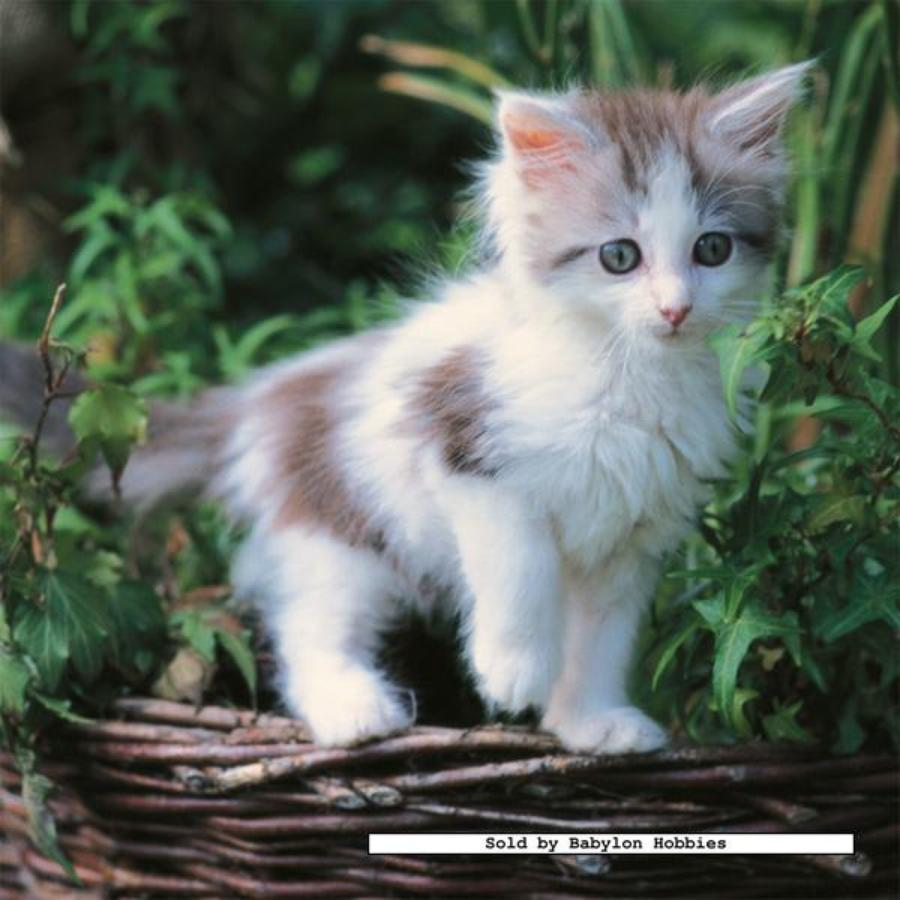
\includegraphics[width=.5\textwidth]{pics/kitten}
\caption{A representation of the pursuit game.}
\label{fig:game}
\end{figure}

\subsubsection{Agent Representation}

Often the pursuit domain is stated as a coevolution problem, with both predators and prey competing to develop better policies. In our approach we focus on the evolution of the predators and the development of coordination strategies.

We use neuro-evolution as the adaptation mechanism for the pursuit domain. Elements of the agent state scaled on the range $[0,1]$ form the input to the neural network. The neural network then has 15 hidden units, and 2 outputs. The first output represents the amount by which the agent chooses to modify its current orientation, $d\theta$, scaled between $[0,2\pi]$. The second output represents the movement length of the agent $dL$, which is scaled between $[0,l_{max}]$, where $l_max=2$ is the maximum value that an agent can choose to move.

An individual $\mathcal{I}$'s state is comprised of $5+N_{\tau}$ different parameters if type information is included, where $N_{\tau}$ is the number of types defined in the system. The first parameter is the absolute orientation $o_{\mathcal{I}}$ of individual $\mathcal{I}$. The second and third are the angle and distance to the nearest prey, $\theta_{prey}$ and $d_{prey}$ respectively. The fourth and fifth elements are the angle and distance to the nearest neighboring pursuer, $\theta_{NN}$ and $d_{NN}$ respectively. The last state elements, which are optionally included based on the setting of the run, are represented by the binary vector $\tau_NN$, which identifies the type of nearest neighbor. These form a tuple $\{o_{me},d_{prey},\theta_{prey},d_{NN}, \theta_{NN},\hat{\tau}_{NN}\}$, which serves as the inputs to the neural network during the run. The distance elements are scaled by an observation radius $d_{limit}=20$, and if the nearest prey or pursuer is outside of this limit it is assigned the maximum limit. The angular elements $o_{me}$, $\theta_{prey}$, and $\theta_{NN}$ are scaled by $2\pi$, unless the prey or pursuer is outside the observational radius, and then this value defaults to 0.

Evolution is performed by mutating a population of $k=10$ neural networks. At each new generation, $k$ new children are created by mutating the parent's weights with a probability $P_{mut}=0.1$, which adds weights by adding a sample from a normal distribution with mean $\mu=0$ and standard deviation $std=1.0$. These $2k$ neural networks are then tested, and assigned a fitness based on the average of $N_{trials}=20$ trials.

We calculate fitness by calculating the distance from the prey at each timestep. We calculate the elemental fitness of an individual $\mathcal{I}$ on trial run $s$:


\[
 TrialFitness(\mathcal{I},s) =
  \begin{cases}
   t_{catch} & \text{if } t_{catch} \leq T \\
   \sum_{t=1}^T \delta(\mathcal{I},t)       & \text{if } t_{catch} > T
  \end{cases}
\]

where $t_{catch}$ is the time required for the pursuer to catch the prey, $\delta(\mathcal{I},t)$ is the distance of individual $\mathcal{I}$ from the nearest prey at time $t$. This is averaged across all trial runs to obtain the fitness of the individual for that epoch:

\begin{equation*}
Fitness(\mathcal{I}) = \sum_{s=1}^{N_{trials}} TrialFitness(\mathcal{I},s);
\end{equation*}





\subsubsection{Types in the Pursuit Game}

We model a set of pursuers with different limitations. These limitations are observable to other pursuers. We define four types of predators in the pursuit game:

\begin{itemize}
\item \textbf{Standard:} A standard-type pursuer has a full range of motion and may turn up to $2\pi$ radians per timestep. At each timestep it may also choose to move forward by a distance of up to $l_{max}$.

\item \textbf{Slow-turning:} A slow-turning type may only turn a maximum of $\pi/2$ radians per timestep. 

\item \textbf{Fast:} The distance selection of a fast agent is scaled by 2. This means that a fast agent can move a maximum of $2 l_{max}$ steps per timestep. Because this merely scales the output, fast-type pursuers retain the capability to move slower per timestep by reducing their neural network output accordingly.

\item \textbf{Erratic:} An erratic-type pursuer evolves a neural controller as the other pursuers but it will with probability $P_{defect}$ select a random angular and distance output not specified by the neural network. This has the same capabilities as a standard-type pursuer.


\end{itemize}

The introduction of heterogeneous types adds an additional dynamic to this domain. A slow-turning agent may not be able to maneuver well toward a prey, and may focus instead on better positioning in order to have the other agents catch the predator.


\subsection{Evasion in the Pursuit Domain}

Capturing prey with random movement provides a relatively easy learning problem for the pursuers, and capture is more likely achieved by chance. We also investigate pursuer response in two cases; one with randomly-moving prey and another with evading prey following a charged particle model. This model set the direction of prey movement, with unit magnitude.

\subsection{The Rover Domain}




\section{Results}
\label{sec:results}

\subsection{Agent Coordination}

To test whether our approach increases the ability of agents to coordinate with one another, we vary the parameters of the predator prey domain. The ratio of predators in this domain dictates whether it is a coordination problem or a congestion problem. In Figure \ref{fig:ratio} we can see that as the number of prey increases in comparison to the predators, the value of the type information becomes greater. 

\begin{figure}[h!]
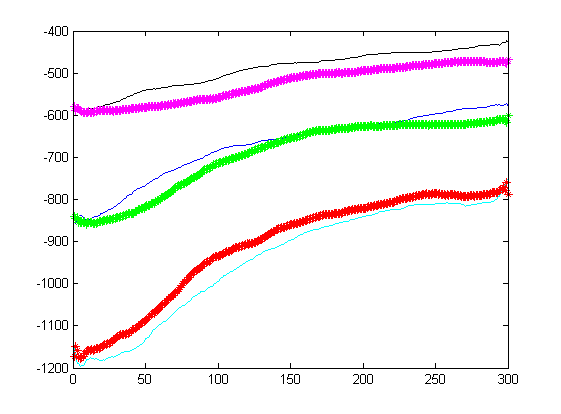
\includegraphics[width=.5\textwidth]{pics/ratio_20a}
\caption{This shows the impact of increasing the ratio of predator to prey in the predator-prey domain.}
\label{fig:ratio}
\end{figure}

%In many cases the agent appears to get into the wrong area of the search space with agents and is not able to escape. For this reason, we train first without observing types, and then at epoch $t=100$ in the simulation types become observable. This addition adds an array of nodes that observe the type of the agent, with randomly generated weights. Because the nodes are added near convergence of the simulation, the weights of the nodes are set to be $\frac{1}{10}$ the size of the weights created at initialization. We show the impact of this delay in Figure \ref{fig:delayimpact}.


%\begin{figure}[h!]
%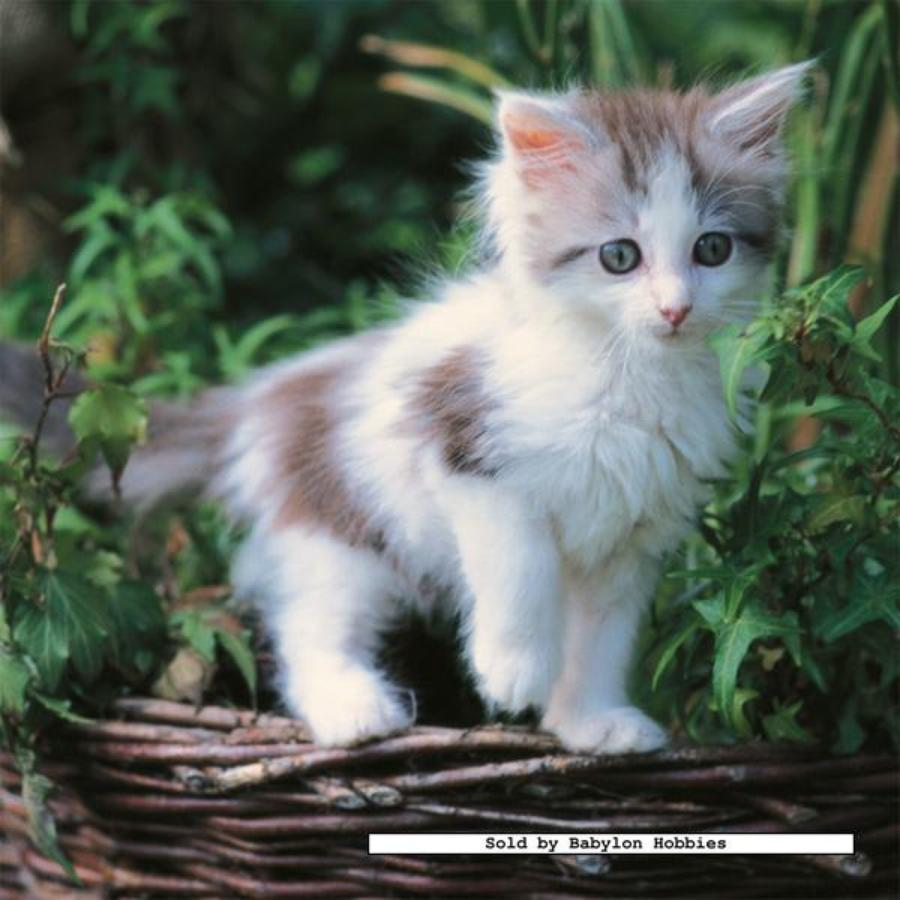
\includegraphics[width=.5\textwidth]{pics/kitten}
%\caption{This shows the average capture times for several different prey evasion strategies.}
%\label{fig:delayimpact}
%\end{figure}

\subsection{Prey Escape Influence}

The type of the prey can also influence the dynamics in the game. We experiment with several different prey types in order to determine the benefits of including a stereotype mechanism with a different learning problem.

\begin{figure}[h!]
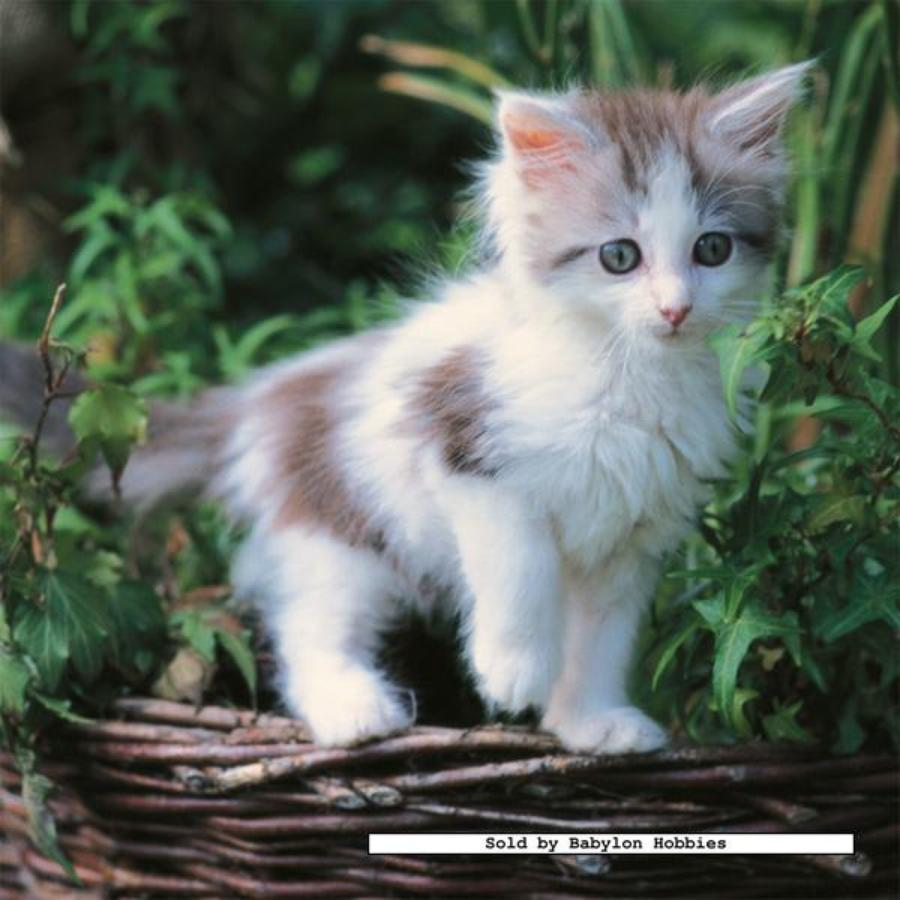
\includegraphics[width=.5\textwidth]{pics/kitten}
\caption{This shows the average capture times for several different prey evasion strategies.}
\label{fig:evasion}
\end{figure}

\subsection{Rover Domain}

We also test the addition of stereotype information in the rover domain. In this domain, a group of rovers must coordinate in order to optimally view points of interest.



\section{Discussion}
\label{sec:discussion}


One of the main insights that this gives us is a look into the nature of roles in the predator-prey domain. The nature of this game changes as the ratio of predators to prey changes. This is because the coordination aspect of the game is increased when there are many predators. It becomes much more important to finding the optimal solution to know \emph{who} you are coordinating with, and a general outline of their capabilities.

Using a neural network for a policy representation offers a mechanism for handling unnecessary information. If the type of the coordinating agent is not helpful, the weights simply decrease during the evolution process to reduce this noise.

Future work involves automatically identifying roles of agents in the system. Even when there are no differences in capability of agents, agents can learn heterogeneous policies in order to solve a model. If these can be characterized they can be used to steer toward better inter-agent coordination.

\bibliographystyle{plain}
\bibliography{AAMAS15}


%
%\subsection{Agent Modeling for Coordination}
%
%Agent modeling has been used primarily in competitive domains, although it has had some applications in teamwork.
%
%\subsection{Coordination Domains}
%
%The points of interest (POI) domain has been explored in several other works \cite{otherstuff}, and is used to highlight the coordination properties of algorithms.
%
%The UAS domain is a real-world domain that the FAA cares about, and can become a difficult coordination problem \cite{faastuff}.
%
%%\subsection{Neuroevolution}
%%We use NEAT to evolve policies.
%
%%NEAT has been used in other works.
%
%
%
%\section{Theoretical Benefit of Stereotypes}
%
%Here we demonstrate using an evolutionary game theoretic model that using a stereotype will improve the converged value of a multiagent reinforcement learning game.
%
%We make some assumptions for this. TODO: outline the assumptions here
%
%We use the replicator dynamics model first presented by Panait and Tuyls in \cite{Panait2007}:
%
%\begin{equation}
%u_i = \sum_{k} a_{ik} y_k
%\end{equation} 
%
%\begin{equation}
%w_j = \sum_k a_{kj} x_k
%\end{equation}
%
%\begin{equation}
%\frac{\frac{dx_i}{dt}}{x_i} = \frac{\alpha}{\tau} (u_i - \sum_k x_k u_k) + \alpha \sum_k x_k \ln{\frac{x_k}{x_i}}
%\end{equation}
%
%\begin{equation}
%\frac{\frac{dy_j}{dt}}{y_j} = \frac{\alpha}{\tau} (w_i - \sum_k y_k w_k) + \alpha \sum_k y_k \ln{\frac{y_k}{y_i}}
%\end{equation}
%
%where $u_i$ is the reward the first agent expects for performing action $i$ and $w_j$ is the reward the second agent expects for taking action $j$.
%
%We can view the formation of partnerships with different agents as a two-player game where an agent is playing with a second agent of mixed strategies. In the case where an agent is type-blind, the strategy must be robust to the possibility that an opponent is playing of either type. However, when the player can observe types or has an accurate internal evaluation of the probability of a strategy type, it can take an action which is more optimal against that playing strategy.
%
%We formalize this by defining our terms...
%
%\begin{itemize}
%\item[] $p_{j,t}$, probability that a collaborating agent $i$ is using strategy type $t$
%\item[] $a_{i,j}$, the payoff of the joint action taken by agent $i$ and $j$
%\item[] BLAH, is some other term we care about
%\end{itemize}
%
%We then show the expected payoff $R_{i,j}$ given that the agent has an unknown mixed strategy:
%
%MATH HERE
%
%We then show the expected payoff $R_{i,j|t}$ given that the agent has a probabilistically known mixed strategy:
%
%MATH HERE
%
%We then show the expected payoff $R^*_{i,j|t}$ where an agent has available strategy type knowledge in each subgame.
%
%
%MATH HERE
%
%We also show that the stereotype identification does not need to be completely accurate; with some probability $p_{wrong,i,j}$ an agent $i$ will misidentify agent $j$.
%
%MATH HERE
%
%
%We have theoretically shown that using stereotype models can increase the expected payoff of the system. This does not take into account the learning speed of the agents. In some cases, if a probability of action selection is similar, the expected payoff gain is not worth the learning speed sacrifice from dividing the problem. We see this issue later in our experiments.
%
%\section{Experimental Setup}
%
%\subsection{Rover POI domain}
%The points of interest (POI) domain provides a testbed for coordination learning.
%
%\section{Results}
%
%\subsection{Stereotypes with Coordinating Rovers}
%
%
%\begin{figure}
%
\includegraphics[width=0.5\textwidth]{pics/box}
%\caption{Rovers learning without types.}
%\label{fig:rovernotypes}
%\end{figure}
%
%In Figure \ref{fig:rovernotypes}, we show the ability of a rover to learn in a POI domain without type differentiation.
%
%\begin{figure}
%
\includegraphics[width=0.5\textwidth]{pics/box}
%\caption{Rovers learning with types.}
%\label{fig:rovertypes}
%\end{figure}
%
%In Figure \ref{fig:rovertypes}, we show that the ability of a rover to learn in a POI domain with type differentiaton is much higher.
%
%The rover domain is a good testbed to demonstrate the efficacy of type inclusion in a coordination domain, but we want to 
%
%\subsection{Stereotypes for UAS Collision Avoidance}
%
%Collision-avoidance is a similar problem to the POI domain except that agents must coordinate to simultaneously optimize their individual paths and to reduce the risk of collision.
%
%\begin{figure}
%
\includegraphics[width=0.5\textwidth]{pics/box}
%\caption{UAS learning without types.}
%\label{fig:uasnotypes}
%\end{figure}
%
%In Figure \ref{fig:uasnotypes}, we show the ability of a rover to learn in a POI domain without type differentiation.
%
%\begin{figure}
%
\includegraphics[width=0.5\textwidth]{pics/box}
%\caption{UAS learning with types.}
%\label{fig:uastypes}
%\end{figure}
%
%In Figure \ref{fig:uastypes}, we show that the ability of a rover to learn in a POI domain with type differentiaton is much higher.
%
%
%\section{Discussion}

\end{document}